\chapter[Tema]{Estudio de caso}
\label{ch:tema}




\section{Selección de herramientas}
Para abordar el estudio del funcionamiento de asignación de recursos dinámica, se requiere de herramientas que permitan verificar la implementación de las diferentes soluciones propuestas. Estas herramientas deben proveer un entorno controlado donde se puedan probar diferentes características para luego generar información que permita ser analizada, y posteriormente generar una hipótesis, para poder explorar las potencialidades y capacidades del o los protocolos estudiados.

Luego de investigar herramientas capaces de realizar la simulación de un protocolo TSCH bajo IPv6, se seleccionaron las siguientes opciones: OMNET++, y 6TiSCH simulator, simuladores únicos capaces de trabajar con el protocolo 6TiSCH. Alternativas que serán comparadas:


\subsection{OMNET++:}

OMNeT++ es un framework de simulación de eventos de código abierto, basado en componentes modulares, escrito en C, basado en componentes, de arquitectura abierta. Es un simulador de ambientes discretos. Su área de aplicación primaria es la simulación de redes de comunicación, y debido a su arquitectura genérica y flexible, ha sido utilizada exitosamente en redes basadas en colas de espera, y arquitectura de hardware. Múltiples modelos de simulación de fuente abierta han sido publicados, en el campo de las simulaciones de internet. Está licenciado bajo ``Academic Public License'', lo cual otorga libertad de distribución bajo las políticas de GNU.

Ya que OMNeT++ provee una arquitectura modular, estos componentes o módulos están programados en C, y C++, para luego ser ensamblados en componentes y modelos mas grandes utilizando un lenguaje de alto nivel (NED). Su soporte de interfaz gráfica, junto a su arquitectura modular permite que las aplicaciones puedan ser incluidas fácilmente en aplicaciones propias. Aunque OMNeT++ no es un simulador en sí, actualmente está ganando popularidad como una plataforma de simulación de redes en la comunidad científica, asi como la industria. OMNeT++ corre bajo plataforma Linux, Unix y Win32 (Windows 2000, y Windows XP).

\subsubsection{Componentes}

Algunos de los componentes principales que conforman a OMNeT++ son, por ejemplo, las bibliotecas de simulación inteligente:

\begin{enumerate}
    \item Compilador para la topología de descripción de lenguaje NED (nedc)
    \item Interfaz gráfica de usuario para la ejecución del simulador, enlaces dentro de las simulaciones ejecutables (Tkenv)
    \item Interfaz al usuario de las líneas de comando de la simulación ejecutada (Cmdenv)
    \item Herramienta de representación gráfica por vectores de gráficas de resultados.
    \item Herramienta de visualización escalar de gráficas de resultados
    \item Herramienta de documentación de modelo.
    \item Utilidades de generación de semillas, creación de archivos, etc.
    \item Documentación, simulaciones de prueba.
\end{enumerate}

La interfaz de OMNeT++ es utilizada junto con la ejecución de la simulación. Su principal uso es mostrar el contenido del modelo de una forma visible para el usuario, para iniciar o detener la simulación, permitir al usuario intervenir y cambiar una variable u objeto dentro del modelo. Esto es importante al momento de depurar un proyecto. El hecho de tener acceso y poder modificar el modelo permite a los usuarios conocer el comportamiento de lo que se modela. Una interfaz gráfica amigable y agradable a la vista permite entender como funciona el simulador, y el modelo internamente.

\subsubsection{Funcionamiento}

Este simulador por si mismo no proporciona ningún componente específico para la simulación de redes de computadoras, ni colas, ni cualquier otra área. En su lugar, estas áreas de aplicación son proporcionadas por varios modelos de simulación y arquitecturas tales como ``Mobility framework'', o ``INET Framework''. Estos modelos son desarrollados completamente independientes a lo que es OMNeT++, y siguen sus propios ciclos.

Lo que OMNeT++ proporciona en sí es una biblioteca clase de C++ que permite la creación de componentes de simulación como módulos simples y canales. También se proporciona la infraestructura para reunir las simulaciones de estos componentes y configurarlos bajo el lenguaje NED, o en un archivo auto ejecutable. Además de esto, proporciona interfaces donde se puede observar y manipular el tiempo de ejecución, o ambientes para la simulación como ``Tkenv'', ``Cmdenv'', también herramientas para facilitar la creación de simulaciones y evaluar sus resultados.\cite{omnet}

\subsubsection{Modelado de IPv6 con OMNeT++}

OMNeT++ permite modelar redes bajo protocolo IPv6 utilizando inicialmente un ambiente gráfico, el cual solamente diseña la estructura básica del modelo a crear, su comportamiento está dado mediante un programa en C++.


\newpage

\subsection{6TiSCH simulator}
Simulador escrito en python específicamente para el protocolo 6TiSCH. Este simulador, desarrollado por un equipo de la IETF permite manejar las variables necesarias utilizadas por 6TiSCH, además de trabajar con los protocolos estrictamente necesarios para 6TiSCH.
Este simulador es un trabajo activo, y en desarrollo por parte del grupo de estandarización IETF. Quienes definen mecanismos para construir, y mantener calendarizadores de comunicación en las redes de internet de las cosas IOT del mañana.

\subsubsection{Protocolos soportados}

Debido a que el simulador 6TiSCH simulator es altamente dedicado, trabaja con los siguientes protocolos:

\begin{enumerate}
    \item IEEE802.15.4e-2012.
    \item RPL.
    \item 6top.
    \item El modelo  de propagación ``pister-hack'' con colisiones.
    \item El modelo de consumo energético tomado de \cite{vilajosana2014realistic}
\end{enumerate}


Luego de comparar las opciones, por sencillez y especificidad se decidió trabajar con 6TiSCH simulator, ya que es un simulador completamente construido para trabajar con este protocolo, además de ser modular.

\section{Diseño de experimento}

Tras tener la certeza de cuál simulador será el que se utilizará, se procede a plantear el problema de investigación, el cual consiste en analizar el desempeño de la red bajo distintos parámetros.

El objetivo del experimento consiste en llegar a una situación que permita verificar o rechazar la hipótesis, la cual permita fijar una meta para trabajar en la mejora del algoritmo de asignación dinámica de celdas utilizada en el protocolo 6TiSCH.

La hipótesis que se tiene que comprobar corresponde al desempeño de las simulaciones bajo distintas condiciones.

El método de experimentación consiste en analizar las variables manejadas por el simulador, y luego realizar simulaciones con los parámetros seleccionados.

Una vez finalizada la simulación, se analizarán los datos resultantes obtenidos para elaborar conclusiones.



\section{Experimentación}
Para comenzar la experimentación con el simulador ``6TiSCH simulator'', se debe conocer el escenario que se simulará. En este caso consistirá en la implementación de cincuenta motes, y simulaciones de umbral de una, cuatro, y ocho celdas. Cada celda consiste en un espacio de una matriz lineal contenida en cada uno de los motes y asignadas a cada vecino en particular, las cuales serán usados para recibir información del nodo vecino antecesor.

La cantidad de celdas asignadas es calculada por el ``algoritmo de estimación de ancho de banda'' del nodo actual hacia el siguiente mientras se mantenga dentro del umbral permitido. El umbral es un parámetro que permite el sobreaprovisionamiento de celdas, comandado por la política de asignación de celdas. En caso que la cantidad de celdas requeridas sea menor a las definidas por el umbral, el algoritmo eliminará las celdas asignadas que sobren con el fin de desocupar recursos. En el caso que la cantidad de celdas requeridas esté dentro del umbral, no se hará nada, y por el contrario, si esta cifra fuera mayor, el algoritmo solicitará asignar mas celdas. 

Luego de recibir la información, el mote añade la información propia generada concatenándola con la información recibida para luego propagarla hacia el nodo sucesor. Este ciclo se repite por cada Mote que recibe la información del anterior. Este mecanismo de asignaciones trabaja utilizando la función de calendarizador Cero (SF0), función con la que se experimentará, y como se mencionó anteriormente, utiliza el método de calendarización ``vecino a vecino''\cite{dujovne-6tisch-6top-sf0-01}.

Cada nodo transmitirá utilizando su potencia máxima (+0 dBm), y una potencia de ruido de -105 dBm. La duración de cada espacio de tiempo será de diez milisegundos, y una cantidad máxima de cinco reintentos. Se seleccionaron estos valores, ya que son los predeterminados por el simulador, y permite comparar con estudios paralelos.

Para ejecutar este simulador hay que recurrir al directorio {\ttfamily /bin/}, donde se ejecuta por consola el archivo ``runSimOneCPU.py'' con el comando:

\begin{ttfamily}
    python runSimOneCPU.py --otfThreshold 1 --gui

\end{ttfamily}


Es necesario destacar que el comando ``--otfThreshold'' y el número que lo precede corresponde al umbral seleccionado, y el comando ``--gui'' permite invocar la interfaz visual, que para efecto de extracción de datos, no presta utilidad alguna, es solamente para visualizar el proceso de simulación.

Para generar simulaciones con los distintos umbrales, al momento de ejecutar la simulación, se generan archivos con la información generada por el simulador. Esta información debe ser graficada o ``ploteada'' con el programa ``plotStuff.py'', ejecutándola con el comando:

\begin{ttfamily}
    python plotStuff.py

\end{ttfamily}

Este programa esta contenido en el mismo directorio que el programa ``runSimOneCPU.py'', y debe ser ejecutado tras cada simulación, ya que cada simulación genera nuevos sets de datos. Cada set de datos ploteados entrega las gráficas que han sido generadas según parámetros analizados, pero agrupadas según umbral de uno, cuatro y ocho.



\newpage


\section{Análisis de resultados}


Una vez generados los sets de datos, se puede realizar el análisis caso a caso del comportamiento de cada proceso bajo sus determinadas condiciones, las cuales se analizarán a continuación:

\subsection{Latencia versus umbral}

        \begin{figure}[h]
        \graphicspath{ {imagenes/agrupadas/} }
        \centering
        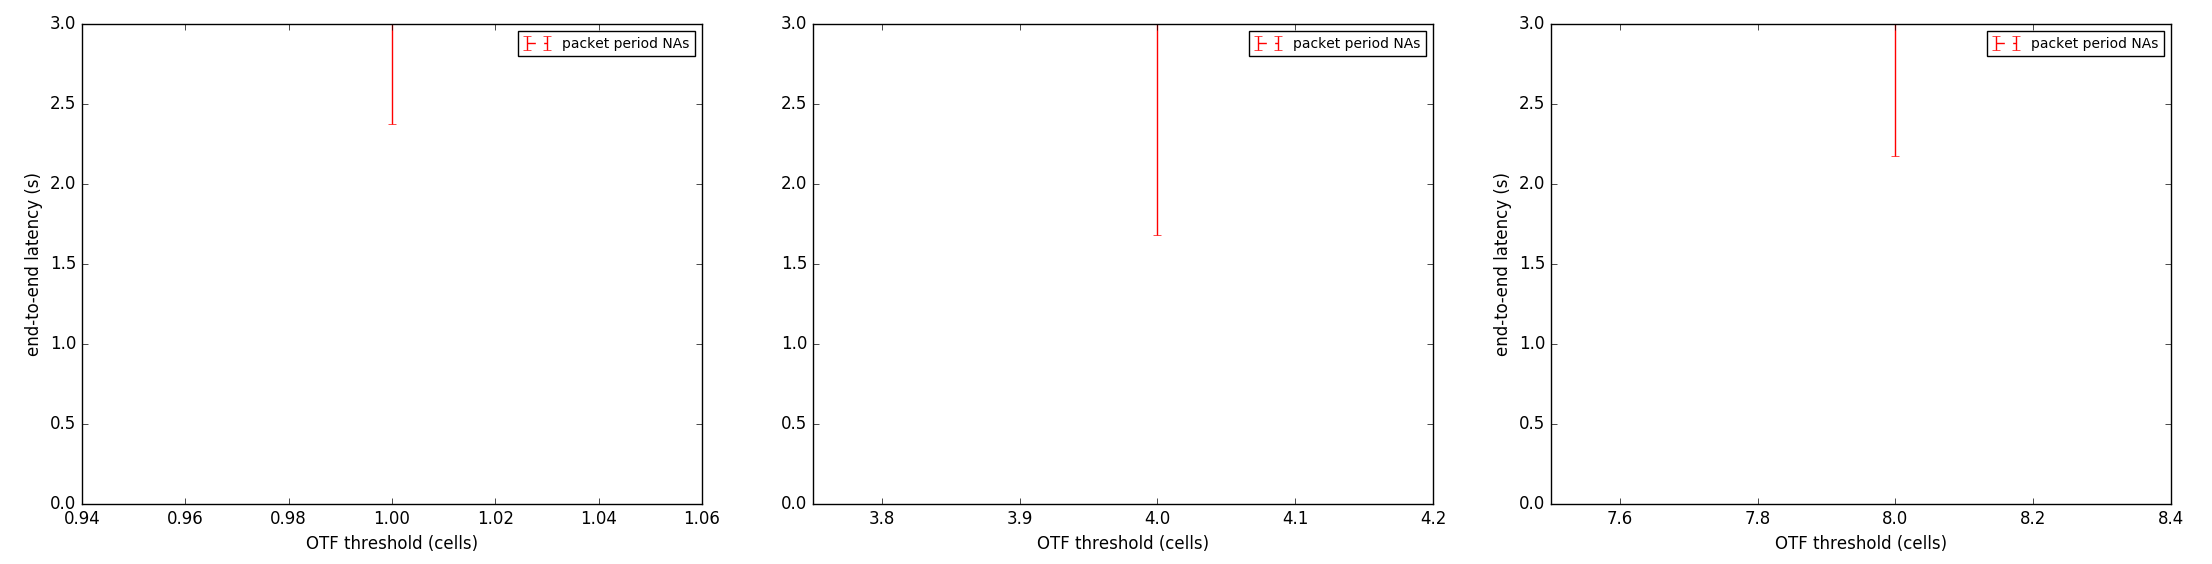
\includegraphics[width=1.0\textwidth]{lat_vs_threshold.png}
        \caption{Lat. vs umbral de 1, 4, y 8 respectivamente}
        \label{latvumbral1}
        \end{figure}


    En las figura \ref{latvumbral1} se muestra las diferencias entre el comportamiento de la latencia según el umbral que se contemple, el umbral que mejor desempeño entrega es con el umbral de cuatro.

\subsection{Latencia versus tiempo}

        \begin{figure}[h]
        \graphicspath{ {imagenes/agrupadas/} }
        \centering
        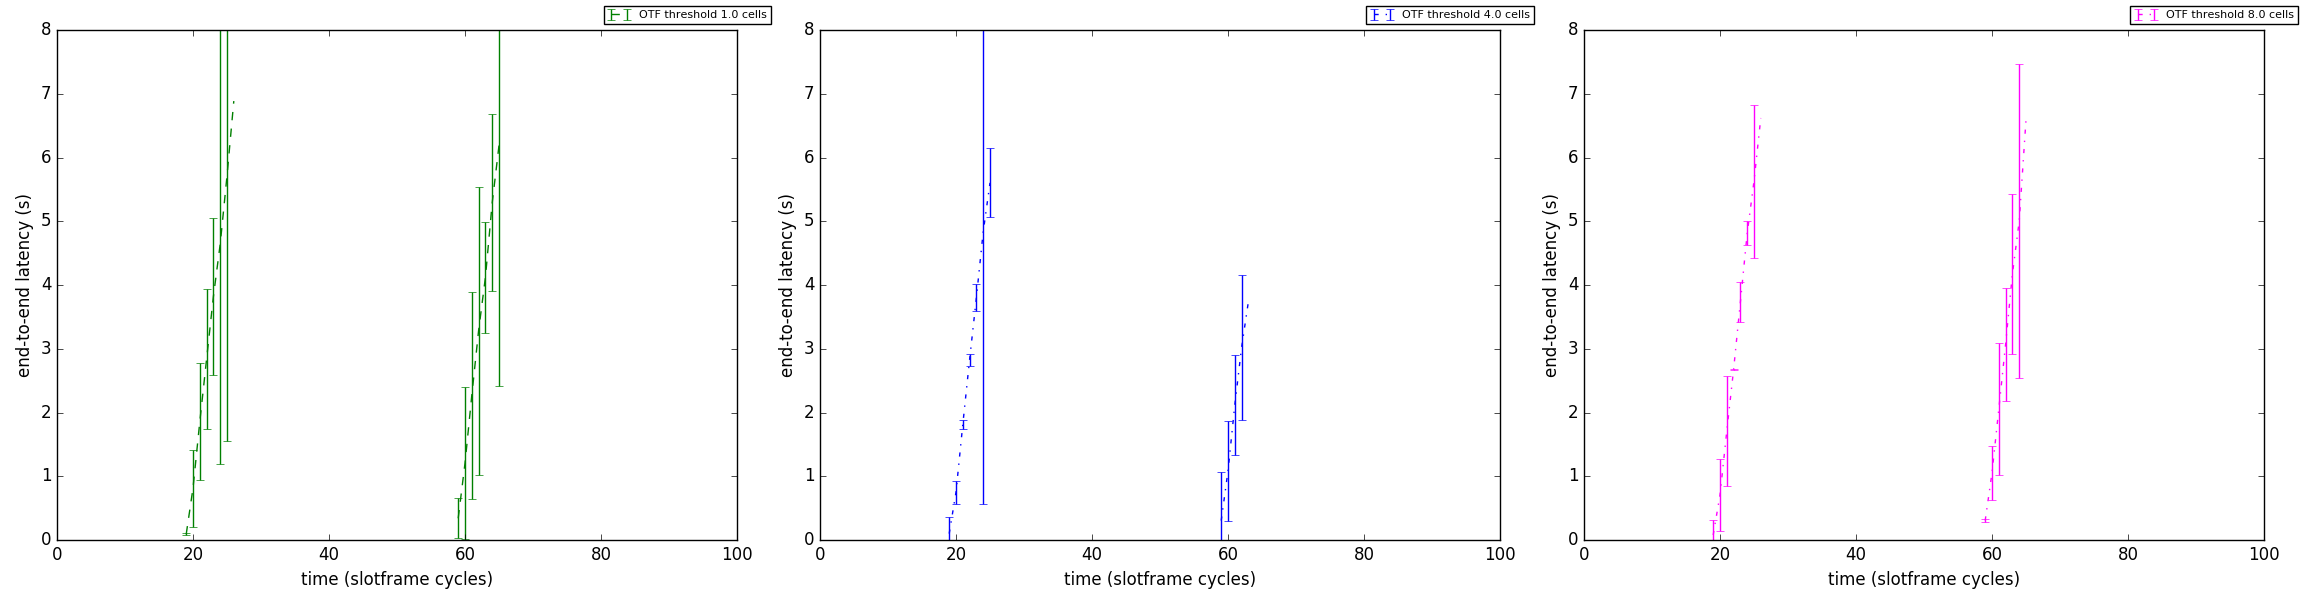
\includegraphics[width=1.0\textwidth]{latvtime.png}
        \caption{Lat. vs tiempo con umbral de 1, 4, y 8 respectivamente}
        \label{latvtime}
        \end{figure}

    Cuando se estudia el comportamiento de la latencia versus el tiempo, graficada en las imágenes agrupadas según umbral \ref{latvtime}. Es posible notar que a mayor umbral, menor propagación de latencia, esto hace sentido, ya que asignar y borrar celdas implican un consumo de tiempo el cual es el requisito de calcular celdas a operar. Es por esto, que la celda con umbral de uno propaga mayor latencia, ya que debe recalcular en mas ocasiones la cantidad de celdas a asignar.
    
    Las asignaciones de celdas versus unidad de tiempo, se pueden ver detalladamente en las imágenes
    
\subsection{Actividad OTF de celdas versus tiempo}

        \begin{figure}[h]
        \graphicspath{ {imagenes/agrupadas/} }
        \centering
        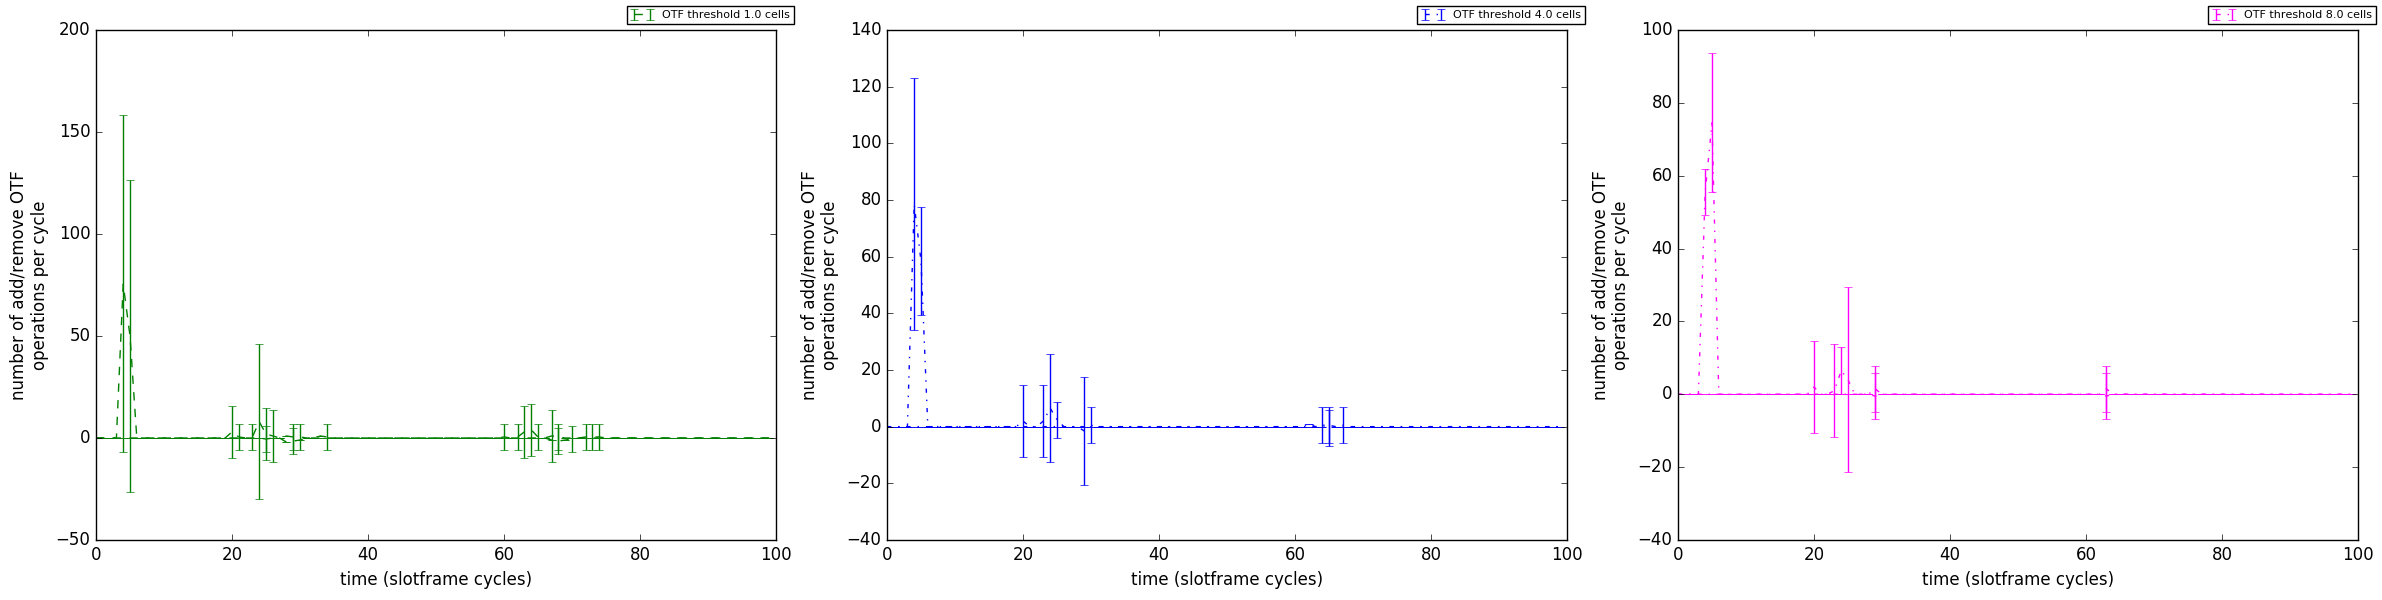
\includegraphics[width=1.0\textwidth]{otfactvstime.png}
        \caption{Activ. OTF con umbral de 1, 4, y 8 respectivamente}
        \label{actotfvtime}
        \end{figure}


    Analizando la actividad ``on the fly'' mostrada en las imágenes \ref{actotfvtime}, es evidente la diferencia del comportamiento según umbral, y que mientras mayor sea el umbral seleccionado, menor será la cantidad de movimientos de asignaciones de celdas de comunicación. Esto es una ventaja, ya que con esto se reduce el consumo energético implicado a las reasignaciones, pero por otro lado, un umbral demasiado grande implica un aumento de latencia, y un consumo excesivo de celdas.
    


\subsection{Número de celdas versus umbral}

        \begin{figure}[h]
        \graphicspath{ {imagenes/agrupadas/} }
        \centering
        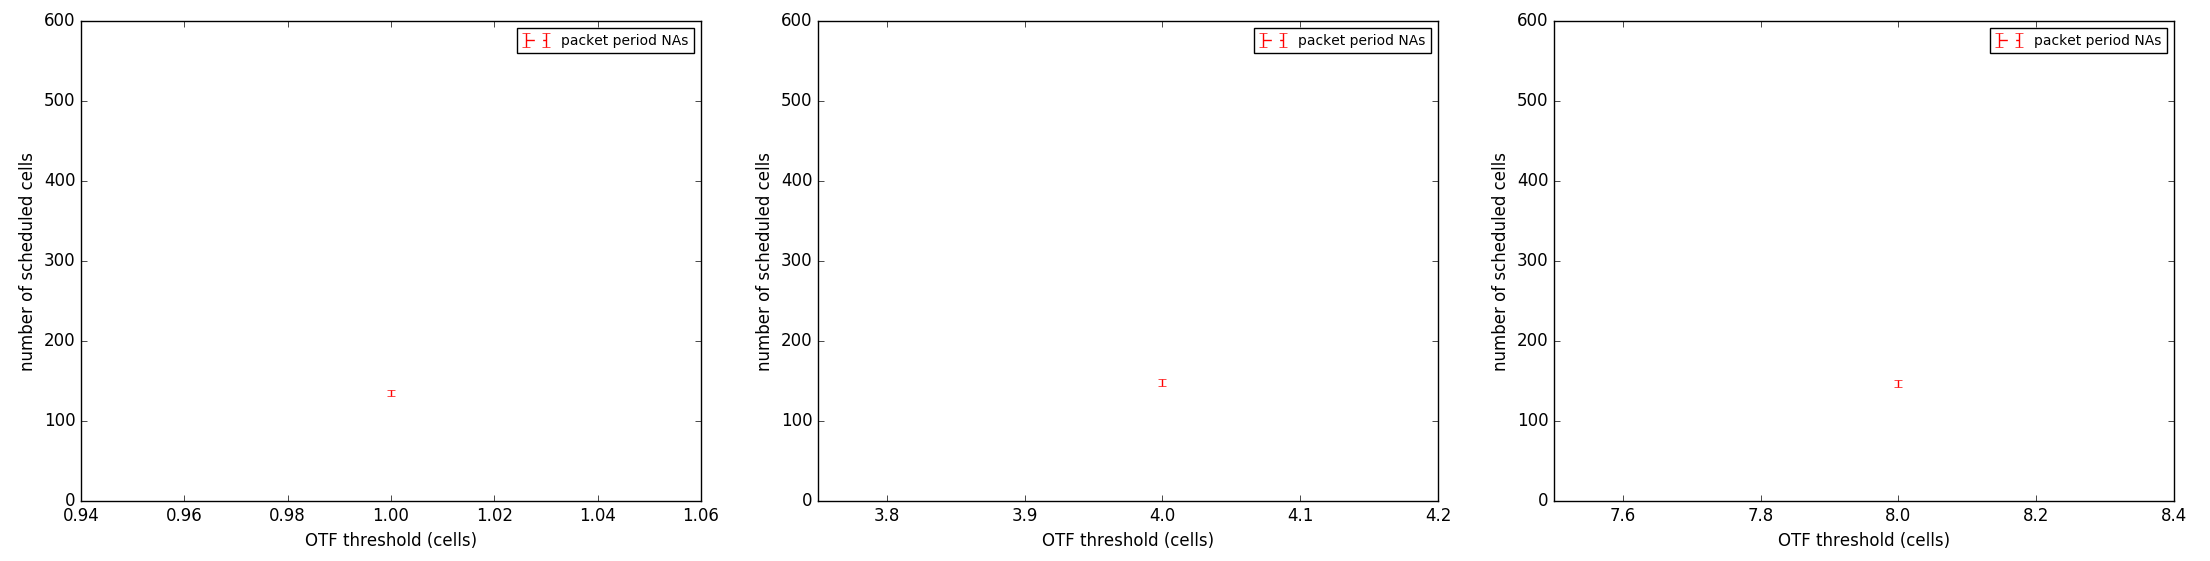
\includegraphics[width=1.0\textwidth]{numcelvsthre.png}
        \caption{Num. de celdas con umbral de 1, 4, y 8 respectivamente}
        \label{numcelvthr}
        \end{figure}

    La cantidad de celdas asignadas reactivamente según umbral tiende a llegar a un equilibrio, en las imágenes \ref{numcelvthr}se puede apreciar que: en la simulación con un umbral de una celda, se tiene una cifra aproximada de ciento veinticinco celdas asignadas, pero al analizar la cifra obtenida por las simulaciones con un umbral de cuatro y ocho, se obtuvo una cifra similar, de alrededor de ciento cincuenta celdas, por lo tanto se puede deducir que se encontró una cifra de equilibrio.


\subsection{Actividad OTF versus umbral}

        \begin{figure}[h]
        \graphicspath{ {imagenes/agrupadas/} }
        \centering
        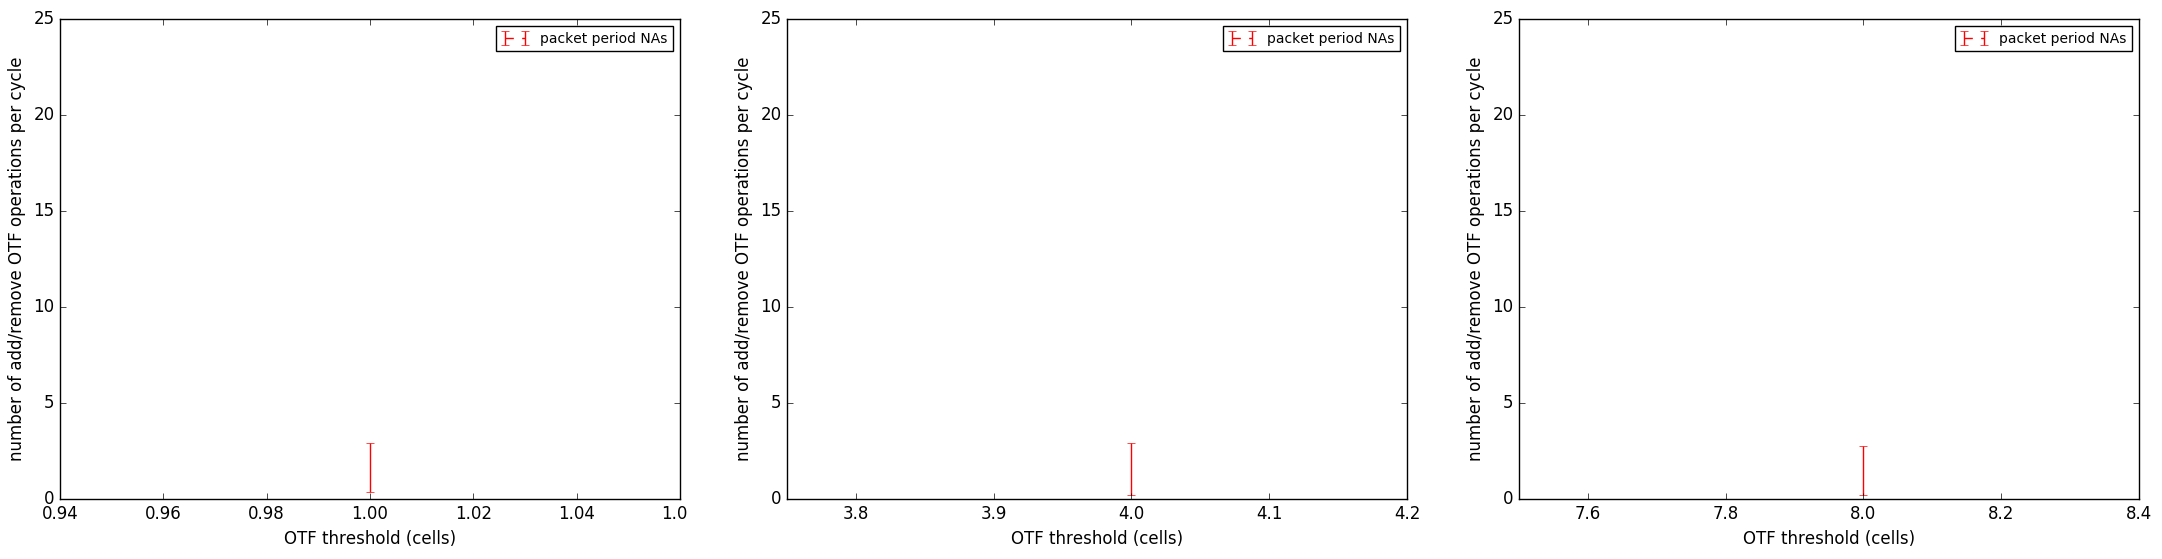
\includegraphics[width=1.0\textwidth]{otfactvthr.png}
        \caption{Act. OTF con umbral de 1, 4, y 8 respectivamente}
        \label{otfactvthr}
        \end{figure}

    La cantidad de operaciones de asignación y eliminado de celdas, tiene un comportamiento similar para cada umbral, las imágenes \ref{otfactvthr} dan cuenta de esto. Por lo tanto con esta información no es posible extraer ninguna conclusión, ya que no hay cambios significativos mas que muy leves diferencias, las cuales pueden ser adjudicadas a factores externos.

\subsection{Comparación de actividad OTF versus tiempo}

        \begin{figure}[h]
        \graphicspath{ {imagenes/agrupadas/} }
        \centering
        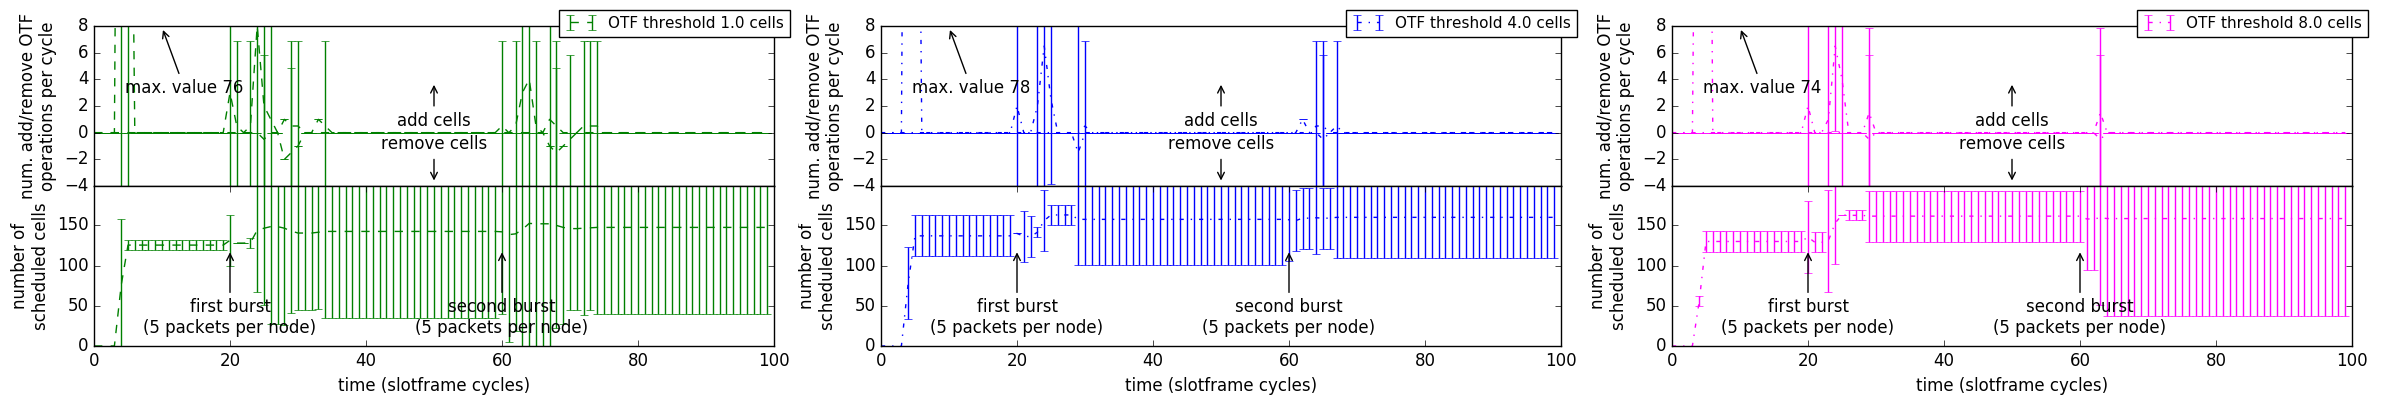
\includegraphics[width=1.0\textwidth]{numcellsotfactivtime.png}
        \caption{Act. OTF vs tiempo con umbral de 1, 4, y 8 respectivamente}
        \label{otfcomp}
        \end{figure}


    Esta sección es crítica, ya que en este momento se ve reflejado el efecto de las diferencias de umbral según sea el caso. Las imágenes \ref{otfcomp} muestra las diferencias en la cantidad de actividad de asignación-borrado de celdas según tamaño de umbral. Esto es coherente con el punto que trata la actividad OTF de celdas versus tiempo, y permite ver en detalle la cantidad de operaciones de asignación-eliminación.
    


\section{Resultados}
    
Al analizar la información de los gráficos generados, se observa que modificando el umbral de la prueba para un tipo de escenario trae consigo una mejora en el desempeño de la prueba, pero esto no implica que mejore el desempeño del proceso general. Por lo tanto analizar un solo gráfico por prueba no permite tener información completa y representativa.

Es necesario trabajar en conjunto con todas las variables según el escenario al que se esté enfrentando. Además de recopilar información respecto al lugar hipotético donde se necesite localizar una malla de sensores, para que junto a un estudio del lugar, permita tomar la mejor decisión respecto a los parámetros con los que trabajarán los nodos.